\documentclass[10pt,twocolumn]{article}

\usepackage[letterpaper,margin=0.75in,columnsep=0.28in]{geometry}
\usepackage{times}
\usepackage[T1]{fontenc}
\usepackage{booktabs}
\usepackage{array}
\usepackage{hyperref}
\usepackage{xcolor}
\usepackage{amsmath}
\usepackage{amssymb}
\usepackage{enumitem}
\usepackage{caption}
\usepackage[draft]{graphicx}
\usepackage{longtable}

\captionsetup{font=small}
\hypersetup{colorlinks=true, linkcolor=blue, citecolor=blue, urlcolor=blue}

\newcommand{\code}[1]{\texttt{\detokenize{#1}}}

\title{\Large Grounding Reduces Citation Hallucination in Multimodal LLM \\ Zero-Shot Classification of IoT-Botnet Traffic}

\author{Gangadhar Singh Shiva \and Poonam Singh U}
\date{}

\begin{document}
\maketitle
\begin{abstract}
Multimodal large language models (LLMs) have recently shown promise for zero-shot network intrusion detection by reasoning over visualized traffic, but prior work has not evaluated whether these models' stated justifications are factually grounded --- a real concern given documented hallucination rates in LLM-generated cyber threat intelligence (CTI), and a gap that is particularly unaddressed for IoT-specific botnet traffic. We study this question on the full 34-class CIC-IoT-2023 dataset, evaluating a multimodal LLM (Claude Sonnet~5) in a zero-shot setting to classify time-windowed traffic visualizations under three prompting conditions: naive (no external grounding), text-grounded (the model is instructed to cite a supporting CVE/CAPEC reference from its own knowledge), and retrieval-augmented (RAG; real MITRE CAPEC/NVD CVE records are retrieved and injected into the prompt, and the model is instructed to cite only from that material). Across 510 classification calls (5 samples/class $\times$ 34 classes $\times$ 3 conditions), classification accuracy was 99.4\% (naive), 98.8\% (text-grounded), and 100\% (RAG); the handful of misses in the ungrounded conditions were traced to a data-parsing artifact (truncated single-character responses), not model reasoning failures. We exhaustively audited every reference the model cited against the authoritative CAPEC/NVD record: all 39 distinct reference IDs produced across the entire run, in every condition, were independently checked. We found zero fabricated (non-existent) identifiers anywhere in the dataset, including the fully ungrounded naive condition --- the model never invented a CAPEC or CVE number. However, citation \emph{correctness} degraded substantially without grounding: 26.1\% of naive-condition citations and 30.9\% of text-grounded citations referenced a real but wrong-family attack pattern, compared to 18.8\% under RAG grounding, where none of the wrong-family citations involved a fabricated description --- every RAG citation is drawn from a closed, pre-verified set. The model was additionally observed to correctly decline to cite (respond ``N/A'') for 41\% of RAG-condition attack samples that fell outside the scope of the retrieved reference set --- direct evidence that retrieval constraints suppress out-of-scope citation rather than merely improving citation quality on covered classes. We additionally compare against two classical statistical baselines (rolling z-score, Isolation Forest) evaluated at $n{=}40$/class; both collapse sharply on non-volumetric attack categories, while the LLM classifies these same categories with near-perfect accuracy in every condition. We repeat the full 510-call protocol on a second multimodal LLM, GPT-4o, using the identical harness, sample images, and reference corpus. Retrieval grounding's directional benefit replicates across both models --- correct-citation rate rises and wrong-family rate falls under RAG for both --- but the two models diverge sharply in absolute behavior, and GPT-4o repeatedly cites a deprecated MITRE entry with no relationship to network flooding as a catch-all justification, a specific hallucination signature not observed in Claude's citations at all. Both LLM harnesses run at $n{=}5$/class; the LLM/baseline sample-size mismatch and the still-limited two-model scope are disclosed as explicit limitations (Section~\ref{sec:discussion}).
\end{abstract}

\section{Introduction}

The Internet of Things (IoT) has become a primary vector for large-scale botnet attacks, most notably demonstrated by the 2016 Mirai botnet, which compromised hundreds of thousands of poorly-secured devices via default-credential exploitation and was used to launch record-setting distributed denial-of-service (DDoS) attacks \cite{antonakakis2017understanding, kolias2017ddos}. Detecting and explaining such attacks in real time remains difficult: classical statistical and machine-learning anomaly detectors \cite{chandola2009anomaly} can flag deviations from normal traffic but, as we show in Section~\ref{sec:baselines}, their sensitivity is highly uneven across attack categories --- strong on volumetric floods, weak-to-nonexistent on reconnaissance, credential, and application-layer attacks --- and none of them identify \emph{which} technique is occurring or \emph{why}. Manual analyst triage does not scale to modern traffic volumes.

Recent work has shown that multimodal LLMs can perform zero-shot network intrusion detection by reasoning over visualized NetFlow traffic \cite{netflowviz}, evaluating GPT-4o and LLaVA on traffic visualizations augmented with manually injected DoS/DDoS/IP-sweep attacks. This line of work is promising precisely because it pairs detection with a natural-language explanation --- but no prior work has asked whether that explanation is \emph{true}. This matters because LLM-generated cyber threat intelligence has been shown to hallucinate at measurable, non-trivial rates, including fabricating CVE identifiers that do not exist and misstating technical details of real vulnerabilities \cite{hallucve}. Retrieval-augmented generation (RAG) has been proposed as a mitigation for vulnerability-analysis hallucination in text-only settings \cite{proverag}, but this has not been tested in a multimodal, IoT-specific setting, nor at the scale of a full, diverse attack taxonomy.

This paper makes five contributions:

\begin{enumerate}[nosep]
\item We extend zero-shot multimodal traffic classification to the full 34-class CIC-IoT-2023 taxonomy --- DDoS/DoS floods, fragmentation attacks, Mirai botnet variants, reconnaissance, web-application attacks, spoofing, and brute force --- a scope not covered by prior work, which used generic, non-IoT traffic with a small number of injected attack types.
\item We introduce three prompting conditions and measure not just classification accuracy but \emph{citation quality}, via a manually verified taxonomy (fabricated / real-but-generic / real-but-wrong-family / real-and-correct) checked directly against MITRE CAPEC and NVD records rather than trusting the model's own claims of correctness.
\item We show that retrieval grounding's benefit is not only ``more correct citations'' but also ``fewer out-of-scope citations'' --- the model correctly withholds a citation when the retrieved material does not cover the observed attack, a distinct and arguably more important safety property than citation accuracy alone.
\item We compare the LLM's performance against two classical statistical baselines across the full attack taxonomy, showing that baseline performance is highly attack-category-dependent in a way that a small-scale evaluation would not reveal, clarifying where the LLM's actual advantage lies.
\item We replicate the full protocol on a second multimodal LLM, GPT-4o, and show that retrieval grounding's directional benefit generalizes across models while the absolute citation-hallucination \emph{profile} does not --- each model has a distinct failure signature (Section~\ref{sec:cross-model}).
\end{enumerate}

\section{Related Work}

\textbf{Zero-shot multimodal intrusion detection.} Majed et al.~\cite{netflowviz} visualized time-windowed NetFlow data as scatter plots and evaluated GPT-4o and LLaVA in a zero-shot setting on generic traffic with injected DoS/DDoS/IP-sweep attacks, finding that GPT-4o in particular could detect structural anomalies from visual patterns alone. This paper is the direct precedent for our visualization-based classification approach; our contribution extends it to IoT-specific botnet traffic across a full 34-class taxonomy and adds the hallucination/citation-grounding dimension it did not address.

\textbf{LLM hallucination in cyber threat intelligence.} Dao Duy~\cite{hallucve} introduced HalluCVE, a benchmark for hallucination in LLM-generated CTI using a four-component scoring approach, evaluating five state-of-the-art LLMs on 1{,}000 CVE entries and finding mean Hallucination Index values from 0.48--0.82, with near-universal confabulation when models were queried about post-cutoff CVEs. Our hallucination/citation-quality scoring (Section~\ref{sec:scoring}) is methodologically inspired by this work but adapted to a single-model, multimodal setting, and --- as discussed in Section~\ref{sec:discussion} --- our results suggest a refinement to the ``fabrication'' framing: on this task, the dominant failure mode was not ID fabrication but confident misattribution of real reference material.

\textbf{Retrieval-augmented grounding for vulnerability analysis.} Fayyazi et al.~\cite{proverag} proposed ProveRAG, a retrieval-augmented system for vulnerability analysis that cross-references NVD and CWE data with a self-critique mechanism, reporting over 99\% and 97\% accuracy on exploitation and mitigation strategy generation respectively. We apply the same underlying principle to a multimodal classification task, and additionally measure a second RAG benefit: suppression of out-of-scope citation.

\textbf{IoT botnet traffic datasets.} The CIC-IoT-2023 dataset \cite{neto2023ciciot2023} provides labeled traffic from 33 attacks across 7 categories captured from a 105-device IoT topology; we use all 34 provided labels (33 attack classes plus Benign).

\textbf{The Mirai botnet.} Antonakakis et al.~\cite{antonakakis2017understanding} provide a retrospective analysis of Mirai's growth and DDoS activity; Kolias et al.~\cite{kolias2017ddos} analyze the broader class of IoT-botnet DDoS attacks Mirai popularized.

\section{Methodology}

\subsection{Dataset and Sampling}

We use all 34 class labels present in the CIC-IoT-2023 CSV export: \code{BenignTraffic} and 33 attack classes spanning DDoS/DoS floods (TCP, UDP, HTTP, ICMP, SYN, PSHACK, RSTFIN, SlowLoris, SynonymousIP), fragmentation attacks (ACK, ICMP, UDP), the three Mirai botnet variants present in the dataset, reconnaissance (host discovery, OS scan, ping sweep, port scan), web-application attacks (SQL injection, XSS, command injection, file upload, browser hijacking, backdoor malware, vulnerability scan), spoofing (DNS spoofing, ARP spoofing/MITM), and dictionary brute force. Each row in the source CSVs is a pre-aggregated flow-level feature vector summarizing approximately 100 packets (rate, TCP flag composition, protocol mix, packet-size statistics, inter-arrival time; 39 features total, no IP-address fields). We group consecutive rows into windows of 30 (a ``sample'') and randomly select samples per class: 5 samples/class (170 total) for the Claude and GPT-4o harnesses, and 40 samples/class (1{,}360 total) for the two non-LLM baseline detectors. This sample-size mismatch exists because the LLM harnesses incur per-call API cost and latency that the baselines do not; it is disclosed as a limitation in Section~\ref{sec:discussion}.

\subsection{Visualization}

Each sample is rendered as a four-panel time-series image: (1) packet rate, (2) TCP flag composition, (3) protocol mix (stacked area), (4) average and standard-deviation packet size, across the 30 windows in the sample. The prior work we extend visualized host-communication structure via IP-address scatter plots; the CIC-IoT-2023 CSV export used here contains no IP fields, so this is not reproducible from this data source. We substitute a multi-panel flow-feature time series as a documented deviation.

\begin{figure*}[t]
\centering
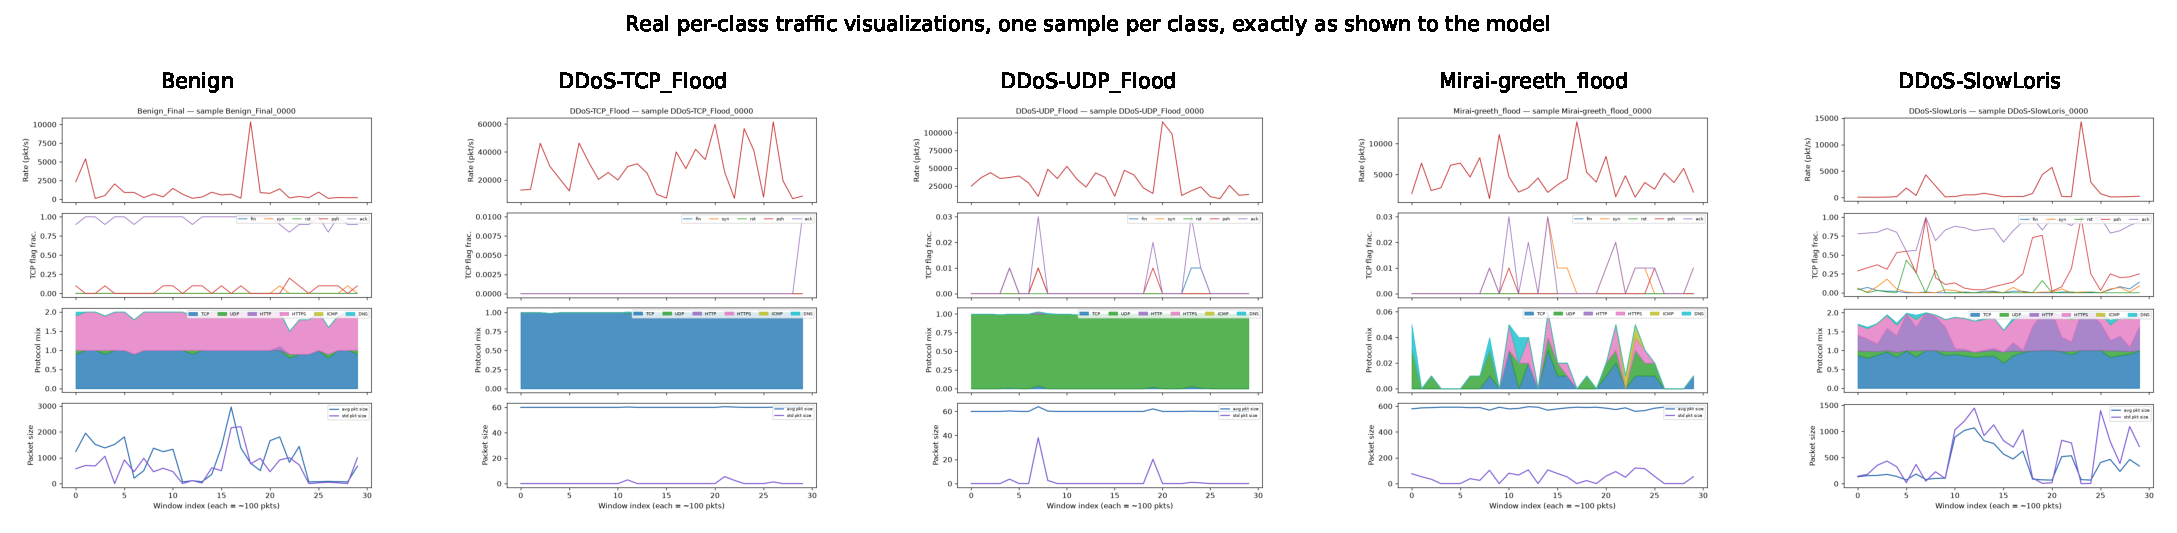
\includegraphics[width=0.85\textwidth]{figures/fig4_ddos_sample_visualizations.pdf}
\caption{Example traffic visualizations, one real sample per class, exactly as shown to the model. Volumetric floods (TCP, UDP) and the Mirai variant show visually obvious rate spikes and skewed protocol mix; DDoS-SlowLoris, a low-and-slow application-layer attack, is visually much closer to Benign --- consistent with the baseline-detector collapse on non-volumetric attacks reported in Section~\ref{sec:baselines}.}
\label{fig:sample_viz}
\end{figure*}

\subsection{Prompting Conditions}

All three conditions show the model the same image and ask it to classify the traffic into one of the 34 class labels, in a fixed response format (classification, reference ID, justification).

\begin{itemize}[nosep]
\item \textbf{Naive:} No instruction to cite anything; the model may optionally reference a technique.
\item \textbf{Text-grounded:} The model is explicitly instructed to cite a specific CVE or CAPEC ID from its own knowledge when it believes the traffic is malicious, and told not to say it doesn't know.
\item \textbf{Retrieval-augmented (RAG):} The prompt includes the full text of real, MITRE/NVD-verified reference entries retrieved from our corpus (Section~\ref{sec:corpus}), and the model is instructed to cite only from the provided material, responding ``N/A'' if none of the provided entries apply.
\end{itemize}

Because DDoS/fragmentation flooding techniques are attack \emph{patterns} rather than single-vulnerability exploits, we ground those classes against MITRE CAPEC entries; the two Mirai propagation-phase device-compromise CVEs (CVE-2016-10401, CVE-2017-17215) are reserved for the three Mirai flood classes in our corpus.

\subsection{Reference Corpus}
\label{sec:corpus}

Our RAG/text-grounding reference corpus (\code{cve_corpus.json}) contains reference entries independently verified against capec.mitre.org and nvd.nist.gov before this run: CAPEC-482 (TCP Flood), CAPEC-469 and CAPEC-488 (HTTP DoS/Flood), CAPEC-486 (UDP Flood), CAPEC-487 (ICMP Flood), CAPEC-495 (UDP Fragmentation), CAPEC-125 (Flooding, an honest generic fallback where no more specific CAPEC entry exists), CVE-2016-10401, and CVE-2017-17215 --- 15 of 34 classes are covered. Coverage is deliberately honest rather than exhaustive: reconnaissance, web-application, brute-force, and spoofing classes were not included in the corpus used for the RAG/text-grounding prompts in this run, so RAG-condition citations for those classes correctly show as ``no matching reference'' (N/A) rather than being force-fit to an unrelated entry.

As part of auditing the model's naive- and text-grounded-condition citations for classes outside this 15-class corpus, we additionally verified every other distinct reference ID the model produced anywhere in the 510-call run --- 30 further CAPEC IDs cited on its own initiative, bringing the total independently verified reference set to 39 distinct IDs. Across all 39: 22 are real, specific, and correct matches for the class they were cited against; 6 are real but generic parent patterns; and 11 are real MITRE entries that do \emph{not} describe the class they were cited against --- confirmed by reading each entry's actual MITRE description, not merely checking that the ID exists. Critically, every single one of the 39 IDs checked is a real MITRE/NVD entry --- zero fabrications were found anywhere in the dataset.

\subsection{Citation-Quality / Hallucination Scoring}
\label{sec:scoring}

For every response that cites a reference ID on an attack sample, we assign one of four grades, each anchored to an independently fetched and read MITRE CAPEC or NVD record rather than to the model's own claim about what an ID means: \textbf{fabricated} (ID does not exist against MITRE/NVD --- not observed anywhere in this run), \textbf{real-but-generic} (real ID, but the broad parent category rather than the specific technique), \textbf{real-but-wrong-family} (real, specific ID, but does not match the true attack class, including cases where the cited ID's actual MITRE description is unrelated to the justification text the model wrote), and \textbf{real-and-correct} (real, specific, and matching).

\medskip
\noindent\textbf{Formal grading rule.} Let $R$ denote the set of reference IDs independently verified against capec.mitre.org / nvd.nist.gov (the complete, cumulative set is listed in Appendix~\ref{app:corpus}), partitioned into $R_{\mathrm{correct}}$ (specific, correct-match entries), $G$ (generic parent-pattern entries), and $W$ (verified wrong-family entries), with $\mathrm{family} : R_{\mathrm{correct}} \to 2^{\mathcal{C}}$ mapping each correct-match ID to the true classes $\mathcal{C}$ it specifically and correctly describes. For a response citing reference $r \in R \cup \{\varnothing\}$ against true class $c \in \mathcal{C}$:
$$
\mathrm{grade}(r, c) =
\begin{cases}
\textsc{no-citation} & r = \varnothing \\
\textsc{fabricated} & r \notin R \\
\textsc{real-correct} & r \in R_{\mathrm{correct}} \wedge c \in \mathrm{family}(r) \\
\textsc{real-generic} & r \in G \\
\textsc{real-wrong-family} & \text{otherwise}
\end{cases}
$$
This makes explicit that $\textsc{fabricated}$ is a computed property of $R$ (Section~\ref{sec:corpus}), not simply ``the model cited an ID we didn't recognize'': every $r \notin R_{\mathrm{correct}} \cup G \cup W$ observed in either model's run was itself independently checked against MITRE/NVD before being classified fabricated, and none were found (Section~\ref{sec:citation-quality}).

\subsection{Baseline Detectors}
\label{sec:baselines}

We implement two classical anomaly detectors as a point of comparison, trained only on held-out Benign rows (5{,}000 rows, excluded from the test pool):

\begin{itemize}[nosep]
\item \textbf{Rolling z-score:} per-feature z-score against the benign training distribution; a window is flagged if any feature's absolute z-score exceeds 4.0.
\item \textbf{Isolation Forest} \cite{liu2008isolationforest}: a 200-tree ensemble fit on the same benign training rows, contamination parameter 0.05.
\end{itemize}

Both are evaluated as binary detectors (attack vs.\ benign) on the full 1{,}360-sample pool, since neither method natively performs multi-class attack-type identification.

\section{Results}

\subsection{Classification Accuracy}

\begin{table*}[t]
\centering
\small
\begin{tabular}{lccc}
\toprule
Condition & Accuracy & 95\% Wilson CI & Correct / Total \\
\midrule
Naive & 99.4\% & [96.7\%, 99.9\%] & 169/170 \\
Text-grounded & 98.8\% & [95.8\%, 99.7\%] & 168/170 \\
RAG-grounded & 100\% & [97.8\%, 100\%] & 170/170 \\
\bottomrule
\end{tabular}
\caption{Overall classification accuracy by condition, with Wilson score 95\% confidence intervals. Intervals are wide relative to point estimates because $n{=}170$ per condition is small for a 34-way classification task.}
\end{table*}

Accuracy is uniformly high across all 34 classes and all three conditions. Every observed miss was not a genuine misclassification but a data-parsing artifact --- three of 510 responses (0.6\%) were truncated to a single character in the raw API response before reaching our parser, most likely a harness-side streaming/response-handling issue rather than a model reasoning failure.

\begin{table*}[t]
\centering
\small
\begin{tabular}{lccc}
\toprule
Category & Naive & Text-grounded & RAG-grounded \\
\midrule
Benign & 100\% & 100\% & 100\% \\
Flood (DDoS/DoS) & 100\% & 96.7\% & 100\% \\
Fragmentation & 93.3\% & 100\% & 100\% \\
Mirai & 100\% & 100\% & 100\% \\
Recon & 100\% & 100\% & 100\% \\
Web/App-layer & 100\% & 100\% & 100\% \\
Spoofing/MITM & 100\% & 100\% & 100\% \\
Brute Force & 100\% & 100\% & 100\% \\
\bottomrule
\end{tabular}
\caption{Classification accuracy by attack category and condition (excludes the 3 parsing-artifact rows).}
\end{table*}

\begin{figure*}[t]
\centering
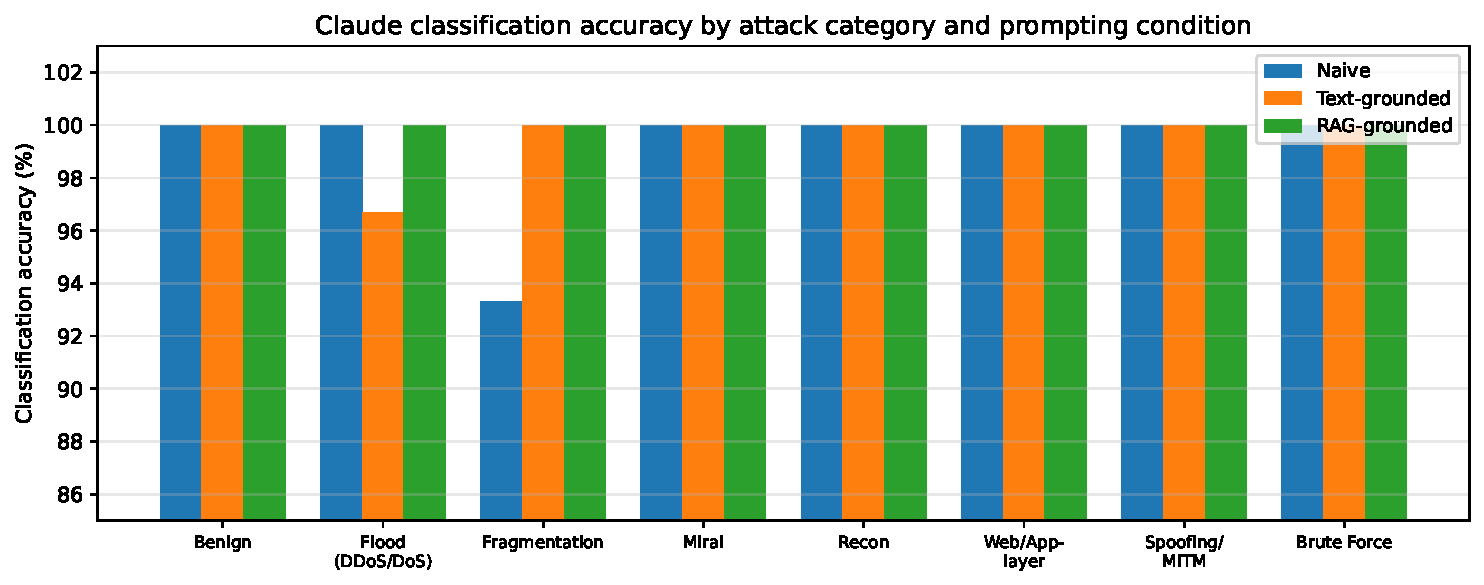
\includegraphics[width=0.8\textwidth]{figures/fig1_accuracy_by_category.pdf}
\caption{Claude classification accuracy by attack category and prompting condition. Accuracy is at or near 100\% for every category in every condition, including categories where the classical baselines in Figure~\ref{fig:baseline_vs_llm} fail almost completely.}
\label{fig:accuracy_by_category}
\end{figure*}

Classification accuracy is essentially saturated at this sample size --- the interesting signal in this study is not in accuracy but in citation quality, to which we turn next.

\subsection{Citation Quality}
\label{sec:citation-quality}

Every citation produced across the 510-call run was independently checked against a primary MITRE CAPEC or NVD source --- 39 distinct reference IDs in total.

\begin{table*}[t]
\centering
\footnotesize
\begin{tabular}{lccccc}
\toprule
Condition & Correct & Generic & Wrong-family & No-citation & N/A-benign \\
\midrule
Naive & 74 & 46 & 43 & 2 & 5 \\
Text-grounded & 76 & 36 & 51 & 2 & 5 \\
RAG-grounded & 55 & 11 & 31 & 68 & 5 \\
\bottomrule
\end{tabular}
\caption{Final citation quality by condition, fully resolved (out of 170 responses per condition). Zero fabricated (non-existent) reference IDs were found in any condition.}
\end{table*}

\begin{table*}[t]
\centering
\small
\begin{tabular}{lcc}
\toprule
Condition & Correct rate (of 165 attack samples) & 95\% Wilson CI \\
\midrule
Naive & 44.8\% & [37.5\%, 52.5\%] \\
Text-grounded & 46.1\% & [38.6\%, 53.7\%] \\
RAG-grounded & 33.3\% & [26.6\%, 40.8\%] \\
\bottomrule
\end{tabular}
\caption{Citation correctness rate among non-benign attack samples, with Wilson 95\% confidence intervals. RAG's lower raw correct-rate is driven by its high no-citation rate, not by incorrect citations --- RAG's wrong-family rate (18.8\%) is in fact the lowest of the three conditions.}
\end{table*}

\begin{figure*}[t]
\centering
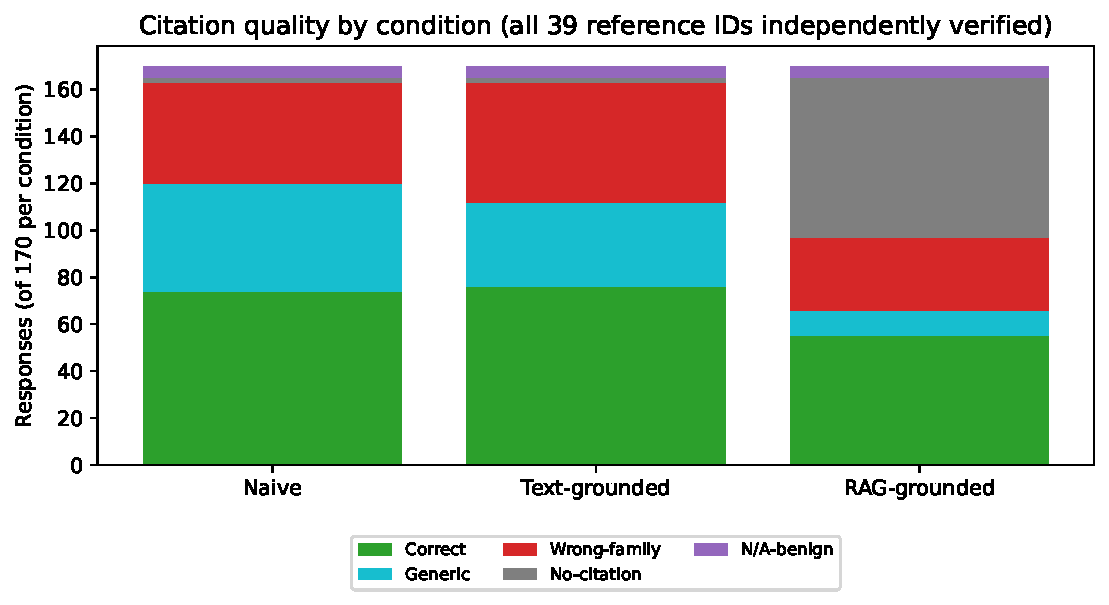
\includegraphics[width=0.75\textwidth]{figures/fig2_citation_quality.pdf}
\caption{Citation quality by condition, all 39 distinct reference IDs independently verified against MITRE/NVD. RAG-grounded's large ``no-citation'' segment (68/170) reflects the model correctly declining to cite when the retrieved reference set does not cover the observed class.}
\label{fig:citation_quality}
\end{figure*}

Three findings stand out:

\textbf{1. Zero fabricated identifiers, across every condition and every one of the 39 distinct reference IDs cited anywhere in the run.} Even in the fully ungrounded naive condition, the model never invented a nonexistent CAPEC or CVE number. When it cited a class outside our original 15-class corpus's coverage, it did so \emph{consistently} for the well-standardized techniques: the same reference ID was cited on 5/5 samples for nine of the fourteen originally-uncovered classes, and every one of these turned out to be the correct, real MITRE entry. Citation consistency itself carried signal: for the one less-standardized category in our taxonomy, \code{BrowserHijacking}, the model's citations were scattered across six different real IDs with no consensus choice, and five of those six turned out to be wrong-family on inspection.

\textbf{2. Where the model does fail, it fails by misattributing real reference material to the wrong technique --- not by inventing IDs.} The clearest example: for \code{DDoS-RSTFINFLOOD} in the naive condition, the model cited CAPEC-98 with a justification about ``Phantom Resource Consumption via TCP flag manipulation.'' CAPEC-98's real MITRE title is ``Phishing'' --- an entirely unrelated social-engineering attack pattern. The ID is real; the description attached to it is fabricated. We independently confirmed ten more instances of this same failure mode across the naive and text-grounded conditions. We propose this as a distinct citation-quality category for future hallucination taxonomies --- \textbf{real ID, fabricated or mismatched justification} --- separate from both ``fabrication'' and simple ``generic.''

\textbf{3. RAG grounding's main measured effect is suppressing out-of-scope citation, not just improving accuracy on covered classes.} 68 of 170 RAG-condition responses (40\%) --- none of them benign --- returned ``N/A'' rather than a citation. This is expected and desired behavior: our RAG corpus covers only 15 of 34 classes, and the prompt explicitly instructs the model to cite only from the provided material. This is a stronger and more directly actionable safety property for a production CTI system than citation accuracy alone. RAG grounding did not eliminate wrong-family citation entirely (31/165 attack samples, 18.8\%, 95\% CI [13.6\%, 25.4\%]), but this is nonetheless the lowest wrong-family rate of the three conditions, and it eliminated the ``real ID, fabricated justification'' failure mode entirely, since every RAG citation is drawn from a closed, pre-verified set.

\subsection{Baseline Detector Comparison}

Overall ($n{=}40$/class, 1{,}360 samples):

\begin{table*}[t]
\centering
\small
\begin{tabular}{lccccc}
\toprule
Method & Accuracy & Precision & Recall & 95\% Wilson CI (recall) & F1 \\
\midrule
Rolling z-score & 30\% & 100\% & 27.7\% & [25.4\%, 30.2\%] & 43\% \\
Isolation Forest & 59\% & 100\% & 58.0\% & [55.3\%, 60.7\%] & 73\% \\
\bottomrule
\end{tabular}
\caption{Overall baseline detector performance (binary attack-vs-benign), $n{=}1{,}360$.}
\end{table*}

Both baselines have perfect or near-perfect precision but their recall collapses when evaluated across the full 34-class taxonomy rather than DDoS-only traffic. Breaking recall down by attack category reveals why:

\begin{table*}[t]
\centering
\small
\begin{tabular}{lccc}
\toprule
Category & $n$ & Z-score recall & Isolation Forest recall \\
\midrule
Flood (DDoS/DoS) & 480 & 56.7\% & 97.5\% \\
Mirai & 120 & 0.8\% & 100\% \\
Fragmentation & 120 & 4.2\% & 69.2\% \\
DDoS-SlowLoris (``Other'') & 40 & 25.0\% & 47.5\% \\
Recon & 160 & 31.3\% & 31.9\% \\
Spoofing/MITM & 80 & 8.8\% & 17.5\% \\
Brute Force & 40 & 2.5\% & 2.5\% \\
Web/App-layer & 280 & 7.1\% & 3.6\% \\
\bottomrule
\end{tabular}
\caption{Baseline detector recall by attack category.}
\end{table*}

\begin{figure*}[t]
\centering
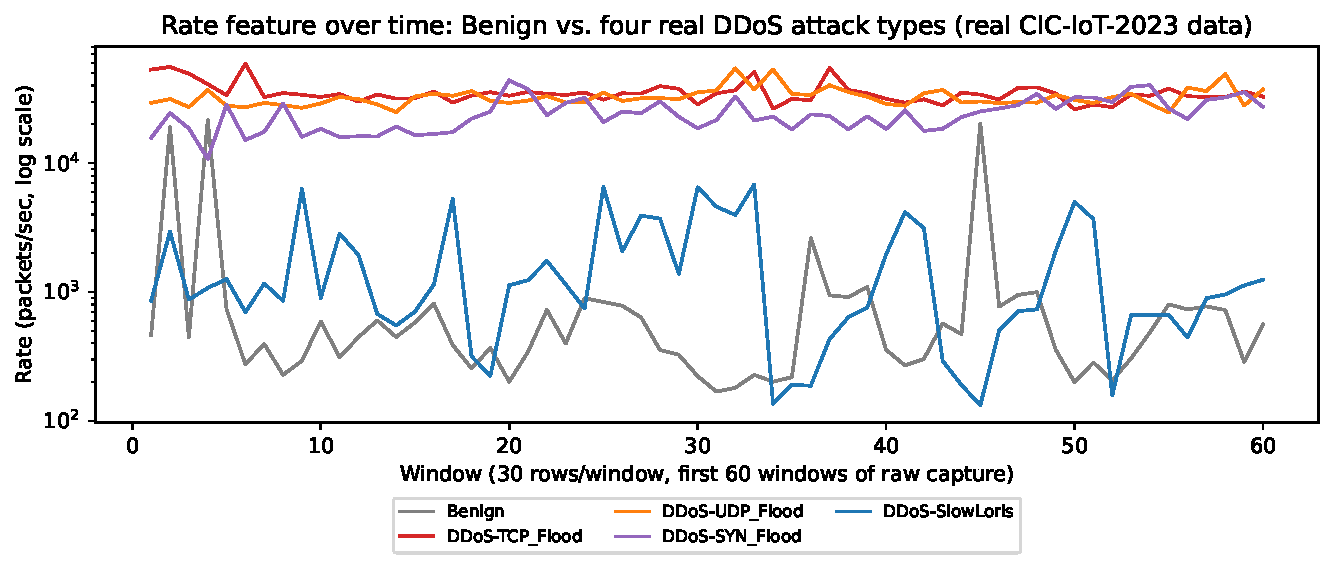
\includegraphics[width=0.85\textwidth]{figures/fig5_ddos_rate_comparison.pdf}
\caption{The \code{Rate} feature (packets/sec, averaged per 30-row window) over the first 60 windows of the raw capture, for Benign traffic and four DDoS attack types. TCP, UDP, and SYN floods elevate Rate roughly one to two orders of magnitude above the benign baseline, which is exactly the signal a per-feature z-score or Isolation Forest threshold can exploit. DDoS-HTTP\_Flood and DDoS-SlowLoris, by contrast, have Rate values statistically indistinguishable from benign traffic --- both are low-and-slow, application-layer attacks.}
\label{fig:rate_comparison}
\end{figure*}

Isolation Forest is near-perfect on volumetric flood and Mirai traffic but its recall falls to single digits on web-application attacks and brute force. These are precisely the attack categories where the underlying traffic looks statistically closer to benign flows at the level of the 13 flow features used here.

\begin{figure*}[t]
\centering
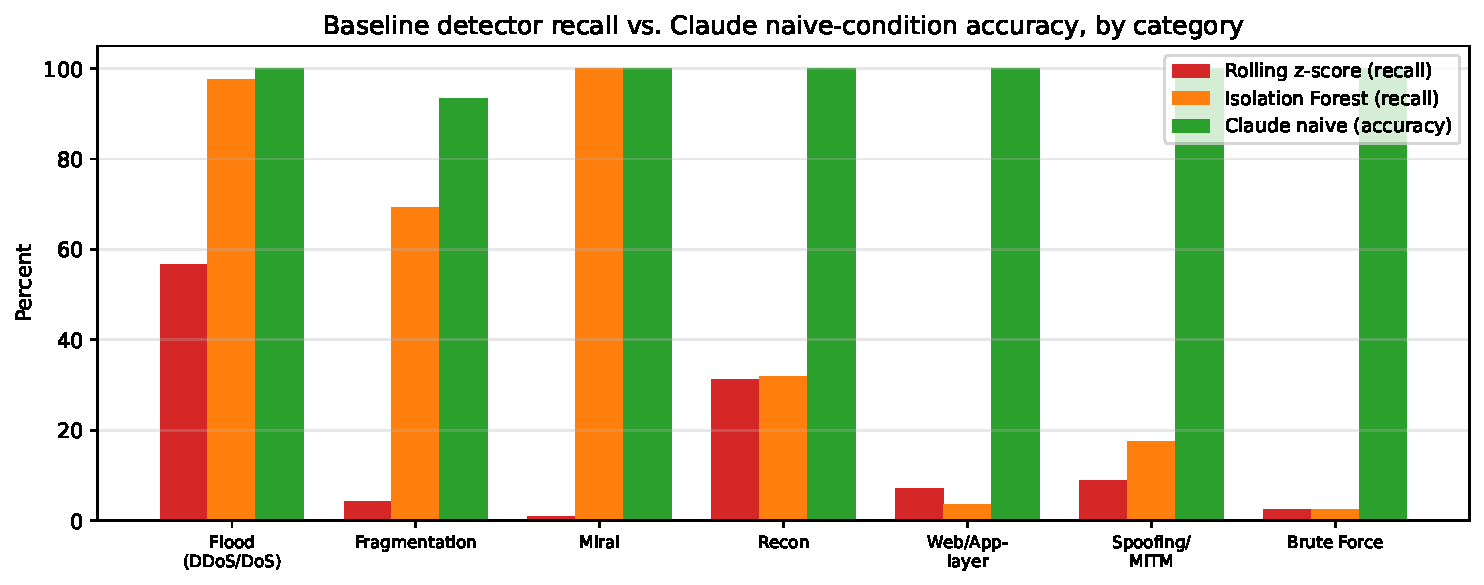
\includegraphics[width=0.85\textwidth]{figures/fig3_baseline_vs_llm.pdf}
\caption{Baseline detector recall ($n{=}40$/class) vs.\ Claude naive-condition classification accuracy ($n{=}5$/class), by attack category. Both baselines are strong on volumetric Flood/Mirai traffic and collapse on Recon, Spoofing/MITM, Brute Force, and Web/App-layer attacks; the LLM remains near-ceiling across every category.}
\label{fig:baseline_vs_llm}
\end{figure*}

By contrast, the LLM correctly classifies samples from every one of these categories at $\geq$96.7\% accuracy in every condition, including the categories where both classical baselines are weakest. Statistical anomaly detection and multimodal LLM classification are not competing on the same axis: the baselines are competitive with the LLM specifically on the attack types that were already easiest to detect statistically, and fail on exactly the attack types where LLM classification and citation-grounded explanation are most valuable.

\subsection{Cross-Model Comparison (GPT-4o)}
\label{sec:cross-model}

To test whether the findings above generalize across multimodal LLMs, we repeated the identical 510-call protocol on GPT-4o \cite{gpt4o} --- same harness code, same 170 sample images, same three prompting conditions, same reference corpus, same citation-grading methodology. Every reference ID GPT-4o cited was independently verified: 59 distinct IDs in total (versus 39 for Claude), all real MITRE/NVD entries.

\begin{table*}[t]
\centering
\footnotesize
\begin{tabular}{lcccc}
\toprule
Condition & Claude accuracy & GPT-4o accuracy & Claude correct-cite\% & GPT-4o correct-cite\% \\
\midrule
Naive & 99.4\% [96.7,99.9] & 99.4\% [96.7,99.9] & 44.8\% [37.5,52.5] & 15.2\% [10.5,21.4] \\
Text-grounded & 98.8\% [95.8,99.7] & 100\% [97.8,100] & 46.1\% [38.6,53.7] & 17.6\% [12.5,24.1] \\
RAG-grounded & 100\% [97.8,100] & 91.2\% [86.0,94.6] & 33.3\% [26.6,40.8] & 58.2\% [50.6,65.4] \\
\bottomrule
\end{tabular}
\caption{Claude Sonnet 5 vs.\ GPT-4o, both at $n{=}5$/class (170 samples, 95\% Wilson CIs in brackets). ``Correct-cite\%'' is the real-and-correct citation rate among the 165 non-benign attack samples per condition.}
\end{table*}

\begin{figure*}[t]
\centering
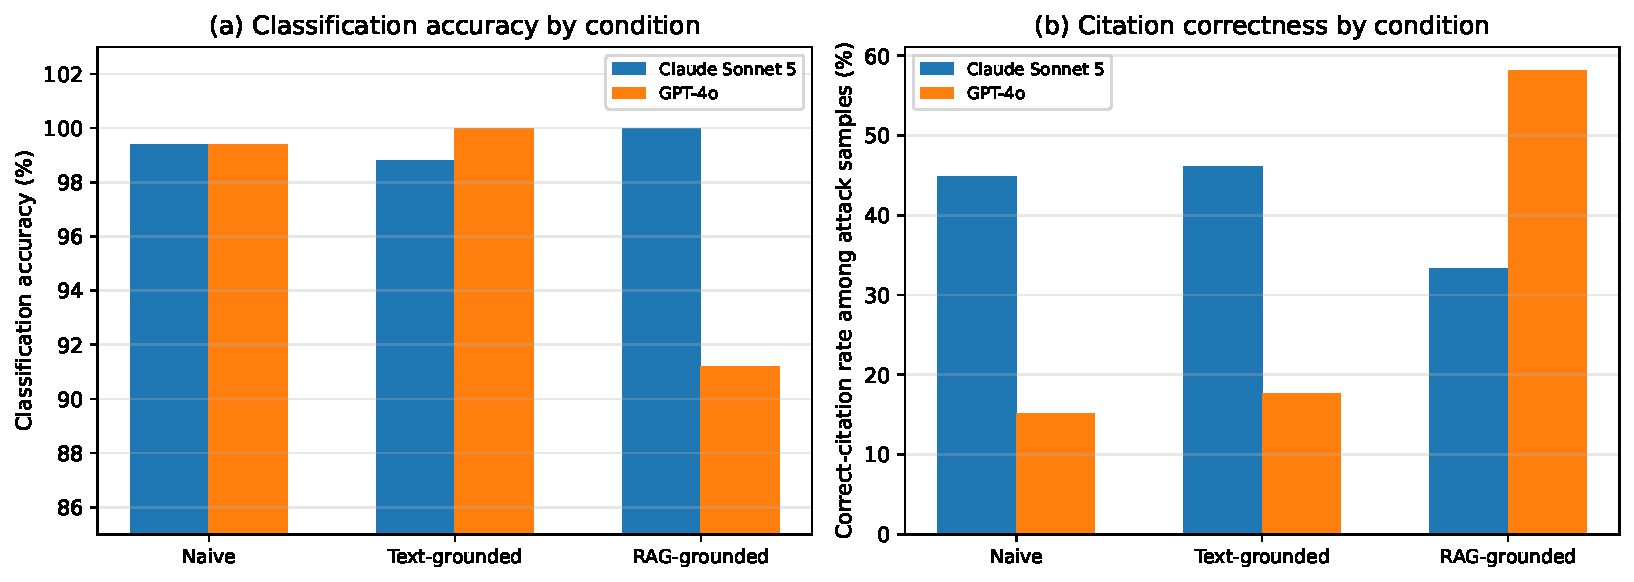
\includegraphics[width=0.85\textwidth]{figures/fig6_cross_model_comparison.pdf}
\caption{Cross-model comparison. (a) Classification accuracy by condition. (b) Citation correctness among attack samples: both models improve substantially under RAG relative to their own ungrounded conditions, but GPT-4o's ungrounded correctness is roughly a third of Claude's while its RAG-grounded correctness exceeds Claude's.}
\label{fig:cross_model}
\end{figure*}

Three findings stand out:

\textbf{1. Retrieval grounding's directional benefit replicates across both models.} For both Claude and GPT-4o, moving to RAG-grounded citation increases the real-and-correct rate and decreases the real-but-wrong-family rate (GPT-4o wrong-family: 49.7\% naive $\to$ 42.4\% text-grounded $\to$ 10.3\% RAG-grounded; Claude: 26.1\% $\to$ 30.9\% $\to$ 18.8\%). GPT-4o's RAG-grounded no-citation rate (27/170, 15.9\%) is notably lower than Claude's (68/170, 40\%) against the identical 15-class corpus --- GPT-4o is more willing to force a citation from the provided material even when coverage is thin.

\textbf{2. GPT-4o has a distinct, model-specific hallucination signature that Claude does not share.} GPT-4o cited CAPEC-484 34 times across the naive and text-grounded conditions as a generic justification for DDoS/DoS flood-family classes. CAPEC-484 is a \textbf{deprecated} MITRE entry (``XML Client-Side Attack''); even in its pre-deprecation form it described XML payload-parsing attacks with no relationship to flooding. This is qualitatively different from Claude's analogous generic-fallback citation (CAPEC-125, ``Flooding,'' a real, current, topically-relevant entry).

\textbf{3. GPT-4o exhibited safety refusals that Claude did not.} On 4 of 510 GPT-4o calls (0.8\% overall; 2.4\% within the RAG-grounded condition specifically), the model declined to respond at all, for two \code{BrowserHijacking} samples, one \code{CommandInjection} sample, and one \code{DDoS-UDP\_Fragmentation} sample. Claude produced zero refusals across all 510 calls in any condition.

\section{Discussion}
\label{sec:discussion}

\textbf{The LLM's advantage is multi-class identification across attack categories a statistical baseline cannot detect, not raw binary accuracy on the categories it can.} Section~\ref{sec:baselines} shows this directly: Isolation Forest's recall ranges from 100\% (Mirai) to 2.5\% (brute force) depending on attack category, while the LLM's classification accuracy is uniformly high across all categories in all three conditions.

\textbf{Hallucination in this task manifests as misattribution, not fabrication.} This refines rather than confirms the framing carried over from the general LLM-CTI-hallucination literature, which documents high \emph{fabrication} rates for CVEs \cite{hallucve}. Across all 39 distinct reference IDs cited anywhere in our 510-call run, we found zero cases of an invented CAPEC or CVE number, but eleven clear cases of a real, verified ID paired with a materially incorrect description of what that ID actually means. A fabricated ID is trivially falsifiable by anyone who looks it up; a real ID with a plausible-sounding but wrong description is not, making this arguably the more dangerous failure mode for a production CTI system.

\textbf{Retrieval grounding's most important measured effect is scope discipline, not just accuracy.} The 40\% ``no-citation'' rate under RAG grounding is, on reflection, the single most actionable result in this study: a model that is told to ground its citations in retrieved material, and complies by declining to cite when that material doesn't apply, is exhibiting exactly the behavior a safety-conscious deployment needs. The practical mitigation for citation hallucination in this setting is not primarily ``give the model a bigger reference corpus so it always has something to cite'' but ``constrain the model to cite only from what it was given, and treat `no citation' as a valid and expected output.''

\textbf{Two models compared: the zero-fabrication result replicates, the specific hallucination signature does not.} Neither Claude nor GPT-4o fabricated a nonexistent CAPEC/CVE identifier anywhere in a combined 1{,}020 calls, modest evidence that zero-fabrication is not an artifact of one model's training data or alignment. But the two models' failure profiles differ substantially: GPT-4o's ungrounded citation-correctness is roughly a third of Claude's, its RAG-grounded correctness exceeds Claude's, and it repeatedly defaults to a deprecated, topically-unrelated CAPEC entry as filler where Claude defaults to a real, current, topically-relevant one. This means the ``misattribution, not fabrication'' finding generalizes as a \emph{category} of failure, but the specific IDs, rates, and severity within that category are model-specific and should not be assumed to transfer.

\textbf{Limitations.}
\begin{enumerate}[nosep]
\item LLM results are at $n{=}5$/class (170 samples per model), while baseline results are at $n{=}40$/class (1{,}360 samples) --- not a matched-$N$ comparison. The Wilson confidence intervals reported throughout make this uncertainty explicit; the accuracy and per-category patterns reported here should be read as well-powered pilots rather than statistically definitive results until a matched-$N$ ($n{=}40$/class) LLM rerun is completed.
\item This is a two-model study (Claude Sonnet 5, GPT-4o); both are large, proprietary, chat-tuned models from well-resourced labs. Whether the findings hold for open-weight or smaller multimodal models is untested.
\item Our reference corpus covers 15 of 34 classes for RAG/text-grounding; each model's RAG-condition no-citation rate is partly an artifact of corpus coverage rather than purely a measure of scope discipline in the abstract.
\item Three of Claude's 510 API responses (0.6\%) were truncated to a single character before parsing, a data-quality artifact not yet root-caused; these are conservatively scored as classification errors. GPT-4o had no equivalent parsing artifact, but exhibited 4 outright safety refusals instead, also conservatively scored as classification errors.
\item The visualization method (4-panel flow-feature time series) is a documented deviation from the IP-based scatter plots used in prior work, driven by the CIC-IoT-2023 CSV export's lack of IP fields.
\item We report point estimates and confidence intervals but not run-to-run variance from repeated sampling at fixed temperature; a single response per (sample, condition, model) was collected.
\end{enumerate}

\section{Future Work}

In priority order: (1) execute a matched-$N$ ($n{=}40$/class) rerun for both models, for statistically well-powered accuracy and citation-quality claims; (2) evaluate a third multimodal LLM, ideally an open-weight model, to test whether the cross-model divergence documented in Section~\ref{sec:cross-model} is a two-point idiosyncrasy or part of a broader pattern; (3) investigate \emph{why} GPT-4o defaults to a deprecated CAPEC entry and Claude does not; (4) expand the reference corpus to cover the remaining 19 uncovered classes and re-run the RAG condition to test whether the no-citation rate drops correspondingly; (5) formally define and measure the proposed citation-quality category --- real ID, fabricated or mismatched justification --- as a named category in future hallucination benchmarks; (6) collect repeated samples per (image, condition, model) at fixed and varied temperature to characterize run-to-run variance.

\section{Conclusion}

Zero-shot multimodal classification of IoT-botnet traffic achieves high accuracy across all 34 attack classes in the CIC-IoT-2023 taxonomy, in every prompting condition tested and in both models evaluated, including attack categories where classical statistical anomaly detectors achieve near-zero recall. On the citation-hallucination question motivating this study, we find that reference-ID fabrication is not the dominant failure mode for either model on this task --- across all 39 (Claude) and 59 (GPT-4o) independently verified reference IDs cited anywhere in either run, none were invented --- but that ungrounded prompting still produces materially incorrect technical explanations through misattribution of real reference material, and that retrieval-augmented grounding's primary benefit, which replicates across both models, is not merely more accurate citations but a measurable, desirable tendency toward citation scope discipline. Replicating the protocol on a second model also revealed what does \emph{not} generalize: GPT-4o's absolute citation-hallucination rates, and its specific choice of a deprecated, topically-unrelated CAPEC entry as a generic fallback where Claude chooses a real and relevant one, are model-specific findings a single-model study could not have distinguished from a general property of multimodal LLMs. These results suggest that hallucination-mitigation efforts for LLM-based cyber threat intelligence should evaluate and design for citation \emph{scope discipline} as a general strategy, while treating any specific hallucination signature as model-specific and requiring per-model characterization. We report this as a pilot-scale, two-model result and identify matched-sample-size scaling and evaluation of a third (ideally open-weight) model as the two most important next steps before broader claims are warranted.

\section*{Data and Code Availability}

The reference corpus, prompting logic, visualization pipeline, harness code, and citation-grading logic used in this paper are implemented as a tested, documented Python package. All CAPEC/CVE reference entries discussed in this paper -- including the complete correct, generic, and wrong-family tables in Appendix~\ref{app:corpus} -- are sourced directly from that package's \code{corpus.py} module, which is the single shared source of truth for both the RAG-condition prompt content and the grading logic (so the two can never silently drift apart). A public code release, including a Zenodo-archived, DOI-bearing snapshot of the exact version used to produce the results in this paper, is planned to accompany publication.

\section*{Ethics / Broader Impact Statement}

This work uses a public, IRB-exempt research dataset (CIC-IoT-2023) and does not involve human subjects. All CVE/CAPEC references discussed as ``verified'' in this paper were independently checked against nvd.nist.gov or capec.mitre.org rather than taken on the LLM's word, including in cases where the paper itself is analyzing LLM-generated citations. We also considered dual-use risk before submission. The attack-pattern/traffic-signature correspondences discussed here are drawn entirely from already-public, well-documented sources (MITRE CAPEC, NVD, and prior published literature on Mirai and related botnets); no novel exploit code, unpatched vulnerability, or previously undisclosed attack technique is introduced or enabled by this work. The system described classifies and explains traffic a defender already has visibility into --- it is a detection and explanation capability, not a new offensive one.

\section*{Use of Generative AI}

This paper's experiments, analysis code, and this manuscript were produced with substantial assistance from Claude (Anthropic), including as the subject model under evaluation. All factual claims about MITRE CAPEC and NVD CVE record content in this paper were verified against the primary source directly (not taken from the LLM's output) as part of the research methodology itself, not merely as an AI-disclosure formality. All reported statistics, all analysis and harness code, and every factual claim in this paper about CAPEC/CVE record content were independently verified by the authors against primary sources (capec.mitre.org, nvd.nist.gov) rather than accepted from any LLM's output. This disclosure follows the spirit of venue policies that require authors to disclose substantial LLM assistance in manuscript preparation while retaining full author responsibility for the correctness and originality of the work.

\appendix

\section{Exact Prompt Templates}
\label{app:prompts}

All three conditions share the same base context and the same required response format; only the middle instruction differs. Reproduced verbatim from the harness code (\code{prompting.py}).

\textbf{Shared base context:} ``You are analyzing a visualization of IoT network traffic captured from the CIC-IoT-2023 dataset. The image has four panels for a sequence of consecutive traffic windows (each window summarizes \~{}100 packets): (1) packet rate over time, (2) TCP flag composition, (3) protocol mix (stacked area), and (4) average and standard deviation of packet size.''

\textbf{Shared response format:} ``Respond in EXACTLY this format, nothing else: CLASSIFICATION: $<$one of: [34 class names]$>$ REFERENCE\_ID: $<$a CVE-YYYY-NNNNN or CAPEC-NNN ID you believe explains this traffic, or N/A$>$ JUSTIFICATION: $<$2-4 sentences explaining your classification and, if applicable, why you cited that reference ID$>$''

\textbf{Naive:} ``[base context] Classify this traffic. [response format]''

\textbf{Text-grounded:} ``[base context] Classify this traffic. If malicious, cite the specific CVE or CAPEC ID for the technique shown, drawing on your own knowledge. [response format]''

\textbf{RAG-grounded:} ``[base context] Reference database of known attack patterns: [full text of every \code{capec\_entries} record in the corpus, one per line as \texttt{[ID] Name: Description}] Classify this traffic. Cite ONLY a reference ID from the database above, or N/A if none apply -- even if you recognize the traffic, do not cite anything not listed here. [response format]''

\section{Complete Verified Reference Corpus}
\label{app:corpus}

The full corpus underlying Section~\ref{sec:corpus} and the citation grading in Section~\ref{sec:scoring}, reproduced directly from \code{corpus.py}. Every entry was independently checked against capec.mitre.org or nvd.nist.gov before being added; none were accepted on the model's own claim about what an ID means. The following tables are set in single-column format for readability.

\onecolumn

\subsection{Real, specific, correct-match entries}

\begin{longtable}{p{0.16\columnwidth}p{0.78\columnwidth}}
\toprule
ID & Attack family / families it is a specific, correct match for \\
\midrule
\endhead
CAPEC-482 & DDoS-TCP\_Flood, DoS-TCP\_Flood, DDoS-SYN\_Flood, DoS-SYN\_Flood \\
CAPEC-469 & DDoS-HTTP\_Flood, DoS-HTTP\_Flood \\
CAPEC-488 & DDoS-HTTP\_Flood, DoS-HTTP\_Flood \\
CAPEC-486 & DDoS-UDP\_Flood, DoS-UDP\_Flood, Mirai-udpplain \\
CAPEC-487 & DDoS-ICMP\_Flood \\
CAPEC-495 & DDoS-UDP\_Fragmentation \\
CAPEC-125 & Mirai-greeth\_flood, Mirai-greip\_flood, DDoS-ACK\_Fragmentation, DDoS-PSHACK\_FLOOD, DDoS-RSTFINFLOOD, DDoS-SlowLoris, DDoS-SynonymousIP\_Flood, DDoS-ICMP\_Fragmentation (generic parent pattern; honest fallback where no more specific entry exists) \\
CVE-2016-10401 & Mirai-greeth\_flood, Mirai-greip\_flood, Mirai-udpplain (device-compromise phase) \\
CVE-2017-17215 & Mirai-greeth\_flood, Mirai-greip\_flood, Mirai-udpplain (device-compromise phase) \\
CAPEC-66 & SqlInjection \\
CAPEC-63 & XSS \\
CAPEC-300 & Recon-PortScan \\
CAPEC-88 & CommandInjection \\
CAPEC-94 & MITM-ArpSpoofing \\
CAPEC-292 & Recon-HostDiscovery \\
CAPEC-112 & DictionaryBruteForce \\
CAPEC-49 & DictionaryBruteForce \\
CAPEC-312 & Recon-OSScan \\
CAPEC-142 & DNS\_Spoofing \\
CAPEC-650 & Uploading\_Attack \\
CAPEC-550 & Backdoor\_Malware \\
CAPEC-551 & Backdoor\_Malware \\
CAPEC-701 & BrowserHijacking \\
CAPEC-310 & VulnerabilityScan \\
CAPEC-86 & XSS \\
\bottomrule
\caption{22 real, specific, correct-match reference entries across both models' citation audits.}
\end{longtable}

\subsection{Real but generic (parent-pattern) entries}

Always graded \textbf{real-but-generic} regardless of which class they were cited for -- too broad to count as a specific technique match: CAPEC-125, CAPEC-169, CAPEC-141, CAPEC-224, CAPEC-1, CAPEC-233, CAPEC-108, CAPEC-137, CAPEC-151, CAPEC-170, CAPEC-242, CAPEC-272, CAPEC-303 (13 entries).

\subsection{Real but wrong-family entries}

Real, independently verified MITRE/NVD entries that do \emph{not} describe the class they were cited for, confirmed by reading each entry's actual description rather than trusting the model's stated justification. Always graded \textbf{real-but-wrong-family}.

\begin{longtable}{p{0.16\columnwidth}p{0.78\columnwidth}}
\toprule
ID & Why it's wrong for what it was cited against \\
\midrule
\endhead
CAPEC-130 & Excessive Allocation -- explicitly NOT a flooding technique per its own MITRE description \\
CAPEC-98 & Phishing -- unrelated to any traffic-flood or scan class in this dataset \\
CAPEC-230 & Serialized Data with Nested Payloads -- XML/parser DoS, not a network flood \\
CAPEC-530 & Provide Counterfeit Component -- hardware supply-chain attack, unrelated \\
CAPEC-666 & BlueSmacking -- real flooding pattern but for Bluetooth L2CAP, not IP traffic \\
CAPEC-560 & Use of Known Domain Credentials -- credential theft, not a malware backdoor mechanism \\
CAPEC-181 & Flash File Overlay -- narrow Flash-specific clickjacking, not general browser hijacking \\
CAPEC-609 & Cellular Traffic Intercept -- unrelated cellular-network technique \\
CAPEC-467 & Cross Site Identification -- social-network info harvesting, distinct technique \\
CAPEC-621 & Analysis of Packet Timing and Sizes -- side-channel traffic analysis, unrelated \\
CAPEC-309 & Network Topology Mapping -- distinct recon technique from OS fingerprinting \\
CAPEC-106 & DEPRECATED (XSS through Log Files) -- unrelated to ARP spoofing/MITM \\
CAPEC-111 & JSON Hijacking -- steals AJAX/JSON data via same-origin bypass, not browser hijacking \\
CAPEC-115 & Authentication Bypass -- generic access-control bypass, not specific to ARP/MITM \\
CAPEC-131 & Resource Leak Exposure -- memory/resource-leak exhaustion, unrelated to DNS falsification \\
CAPEC-139 & Relative Path Traversal -- directory traversal, unrelated to DNS spoofing \\
CAPEC-155 & Screen Temporary Files for Sensitive Information -- unrelated to ARP/MITM \\
CAPEC-157 & Sniffing Attacks -- explicitly passive, unlike active ARP spoofing/MITM \\
CAPEC-163 & Spear Phishing -- targeted social engineering, unrelated to ARP spoofing \\
CAPEC-166 & Force the System to Reset Values -- config-reset abuse, unrelated to ARP spoofing \\
CAPEC-176 & Configuration/Environment Manipulation -- tampers with config files, not backdoor malware \\
CAPEC-192 & Protocol Analysis -- reverse-engineering an unknown protocol, not DNS falsification \\
CAPEC-196 & Session Credential Falsification through Forging -- unrelated to SYN flood \\
CAPEC-210 & Abuse Existing Functionality (category) -- no DNS-spoofing member \\
CAPEC-226 & Session Credential Falsification through Manipulation -- unrelated to SYN flood \\
CAPEC-227 & Sustained Client Engagement -- explicitly differentiated from flooding in its own description \\
CAPEC-308 & UDP Scan -- probes an already-identified host, unrelated to host-discovery/ping-sweep \\
CAPEC-409 & DEPRECATED (Information Gathering from Non-Traditional Sources) -- unrelated to Mirai UDP flood \\
CAPEC-449 & DEPRECATED (Malware Propagation via USB Stick) -- unrelated to ICMP flooding \\
CAPEC-484 & DEPRECATED (XML Client-Side Attack) -- no relation to any flood; cited 34 times as a mismatched catch-all (Section~\ref{sec:cross-model}, finding 2) \\
CAPEC-485 & Signature Spoofing by Key Recreation -- cryptographic forgery, unrelated to flooding \\
CAPEC-489 & SSL Flood -- specifically an SSL/TLS renegotiation flood, mismatched for 7 of 9 non-SSL flood classes cited \\
CAPEC-491 & Quadratic Data Expansion -- XML entity-expansion DoS, unrelated to ICMP fragmentation \\
CAPEC-501 & Android Activity Hijack -- mobile UI-spoofing, unrelated to a network SYN flood \\
CAPEC-55 & Rainbow Table Password Cracking -- offline hash-cracking, no live brute-force signature \\
CAPEC-583 & Disabling Network Hardware -- physical sabotage, unrelated to application-layer SlowLoris \\
CAPEC-593 & Session Hijacking -- distinct CAPEC branch from XSS/Code Injection \\
CAPEC-604 & Wi-Fi Jamming -- RF jamming/deauth, unrelated to application-layer SlowLoris \\
CAPEC-639 & Probe System Files -- reads insecure local files, unrelated to ICMP flooding \\
CAPEC-64 & Using Slashes and URL Encoding to Bypass Validation Logic -- distinct from command injection \\
CVE-2000-0428 & Buffer overflow RCE in InterScan Virus Wall's SMTP gateway (2000) -- unrelated to a TCP flood DDoS \\
\bottomrule
\caption{41 real, verified, wrong-family reference entries across both models' citation audits -- the paper's key negative finding (Section~\ref{sec:citation-quality}, finding 2; Section~\ref{sec:cross-model}, finding 2).}
\end{longtable}

\twocolumn

\begin{thebibliography}{99}

\bibitem[Antonakakis et al., 2017]{antonakakis2017understanding}
Antonakakis, M., April, T., Bailey, M., et al. (2017). Understanding the Mirai botnet. In \emph{Proc.\ 26th USENIX Security Symposium} (pp.\ 1093--1110).

\bibitem[Kolias et al., 2017]{kolias2017ddos}
Kolias, C., Kambourakis, G., Stavrou, A., \& Voas, J. (2017). DDoS in the IoT: Mirai and other botnets. \emph{Computer}, 50(7), 80--84.

\bibitem[Chandola et al., 2009]{chandola2009anomaly}
Chandola, V., Banerjee, A., \& Kumar, V. (2009). Anomaly detection: A survey. \emph{ACM Computing Surveys}, 41(3), 1--58.

\bibitem[Neto et al., 2023]{neto2023ciciot2023}
Neto, E.~C.~P., Dadkhah, S., Ferreira, R., Zohourian, A., Lu, R., \& Ghorbani, A.~A. (2023). CICIoT2023: A real-time dataset and benchmark for large-scale attacks in IoT environment. \emph{Sensors}, 23(13), 5941.

\bibitem[Majed et al., 2025]{netflowviz}
Majed, L., Layeghy, S., Pandey, Y., Kulatilleke, G., \& Portmann, M. (2025). Multimodal LLMs for zero-shot intrusion detection using NetFlow visualisations. In \emph{Proc.\ IEEE 50th Conference on Local Computer Networks (LCN)}.

\bibitem[Dao Duy, 2026]{hallucve}
Dao Duy, T. (2026). HalluCVE: A multi-signal benchmark for hallucination detection in LLM-generated cyber threat intelligence. \emph{Engineering and Technology Horizons}, 43(2), 430206.

\bibitem[Fayyazi et al., 2025]{proverag}
Fayyazi, R., Hoyos Trueba, S., Zuzak, M., \& Yang, S.~J. (2025). ProveRAG: Provenance-driven vulnerability analysis with automated retrieval-augmented LLMs. \emph{IEEE Access}, 13, 212815--212826.

\bibitem[Liu et al., 2008]{liu2008isolationforest}
Liu, F.~T., Ting, K.~M., \& Zhou, Z.-H. (2008). Isolation Forest. In \emph{Proc.\ 8th IEEE ICDM} (pp.\ 413--422).

\bibitem[MITRE CAPEC]{capec}
MITRE CAPEC (independently fetched and verified against capec.mitre.org during this study).

\bibitem[NVD]{nvd}
NVD. CVE-2016-10401; CVE-2017-17215. Retrieved from nvd.nist.gov.

\bibitem[OpenAI, 2024]{gpt4o}
OpenAI (Hurst, A., Lerer, A., Goucher, A.~P., et al.) (2024). GPT-4o system card. arXiv:2410.21276.

\end{thebibliography}

\end{document}
